\providecommand{\main}{../../../..}
\documentclass[\main/dresen_thesis.tex]{subfiles}
\begin{document}
  \label{sec:looselyPackedNS:bilayerStacks:gisaxs}
  \begin{figure}[tb]
    \centering
    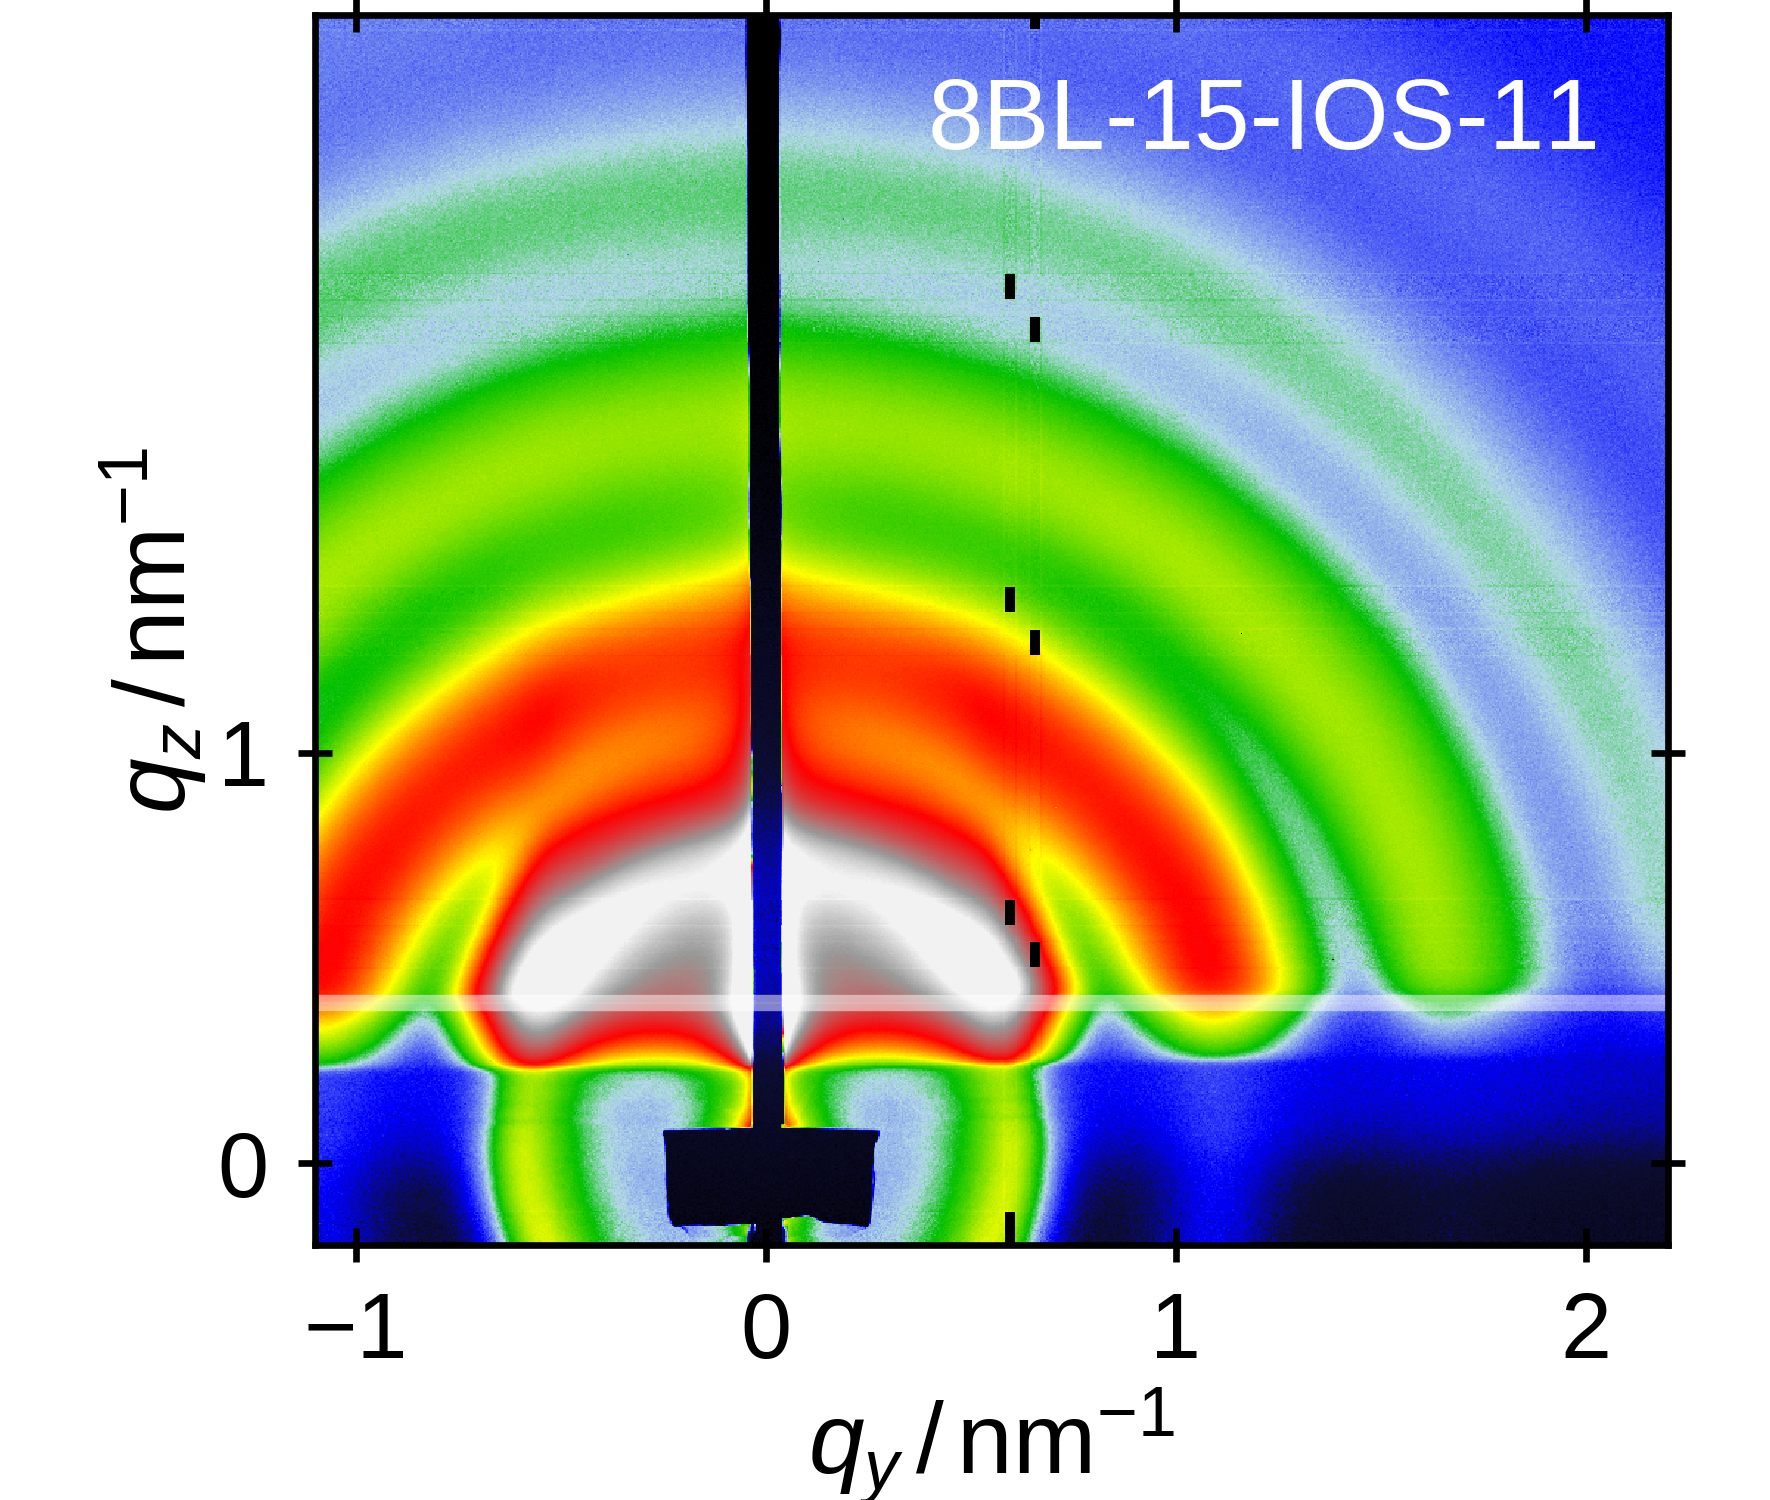
\includegraphics{looselyPackedNP_GISAXS_8BL-15-IOS-11}
    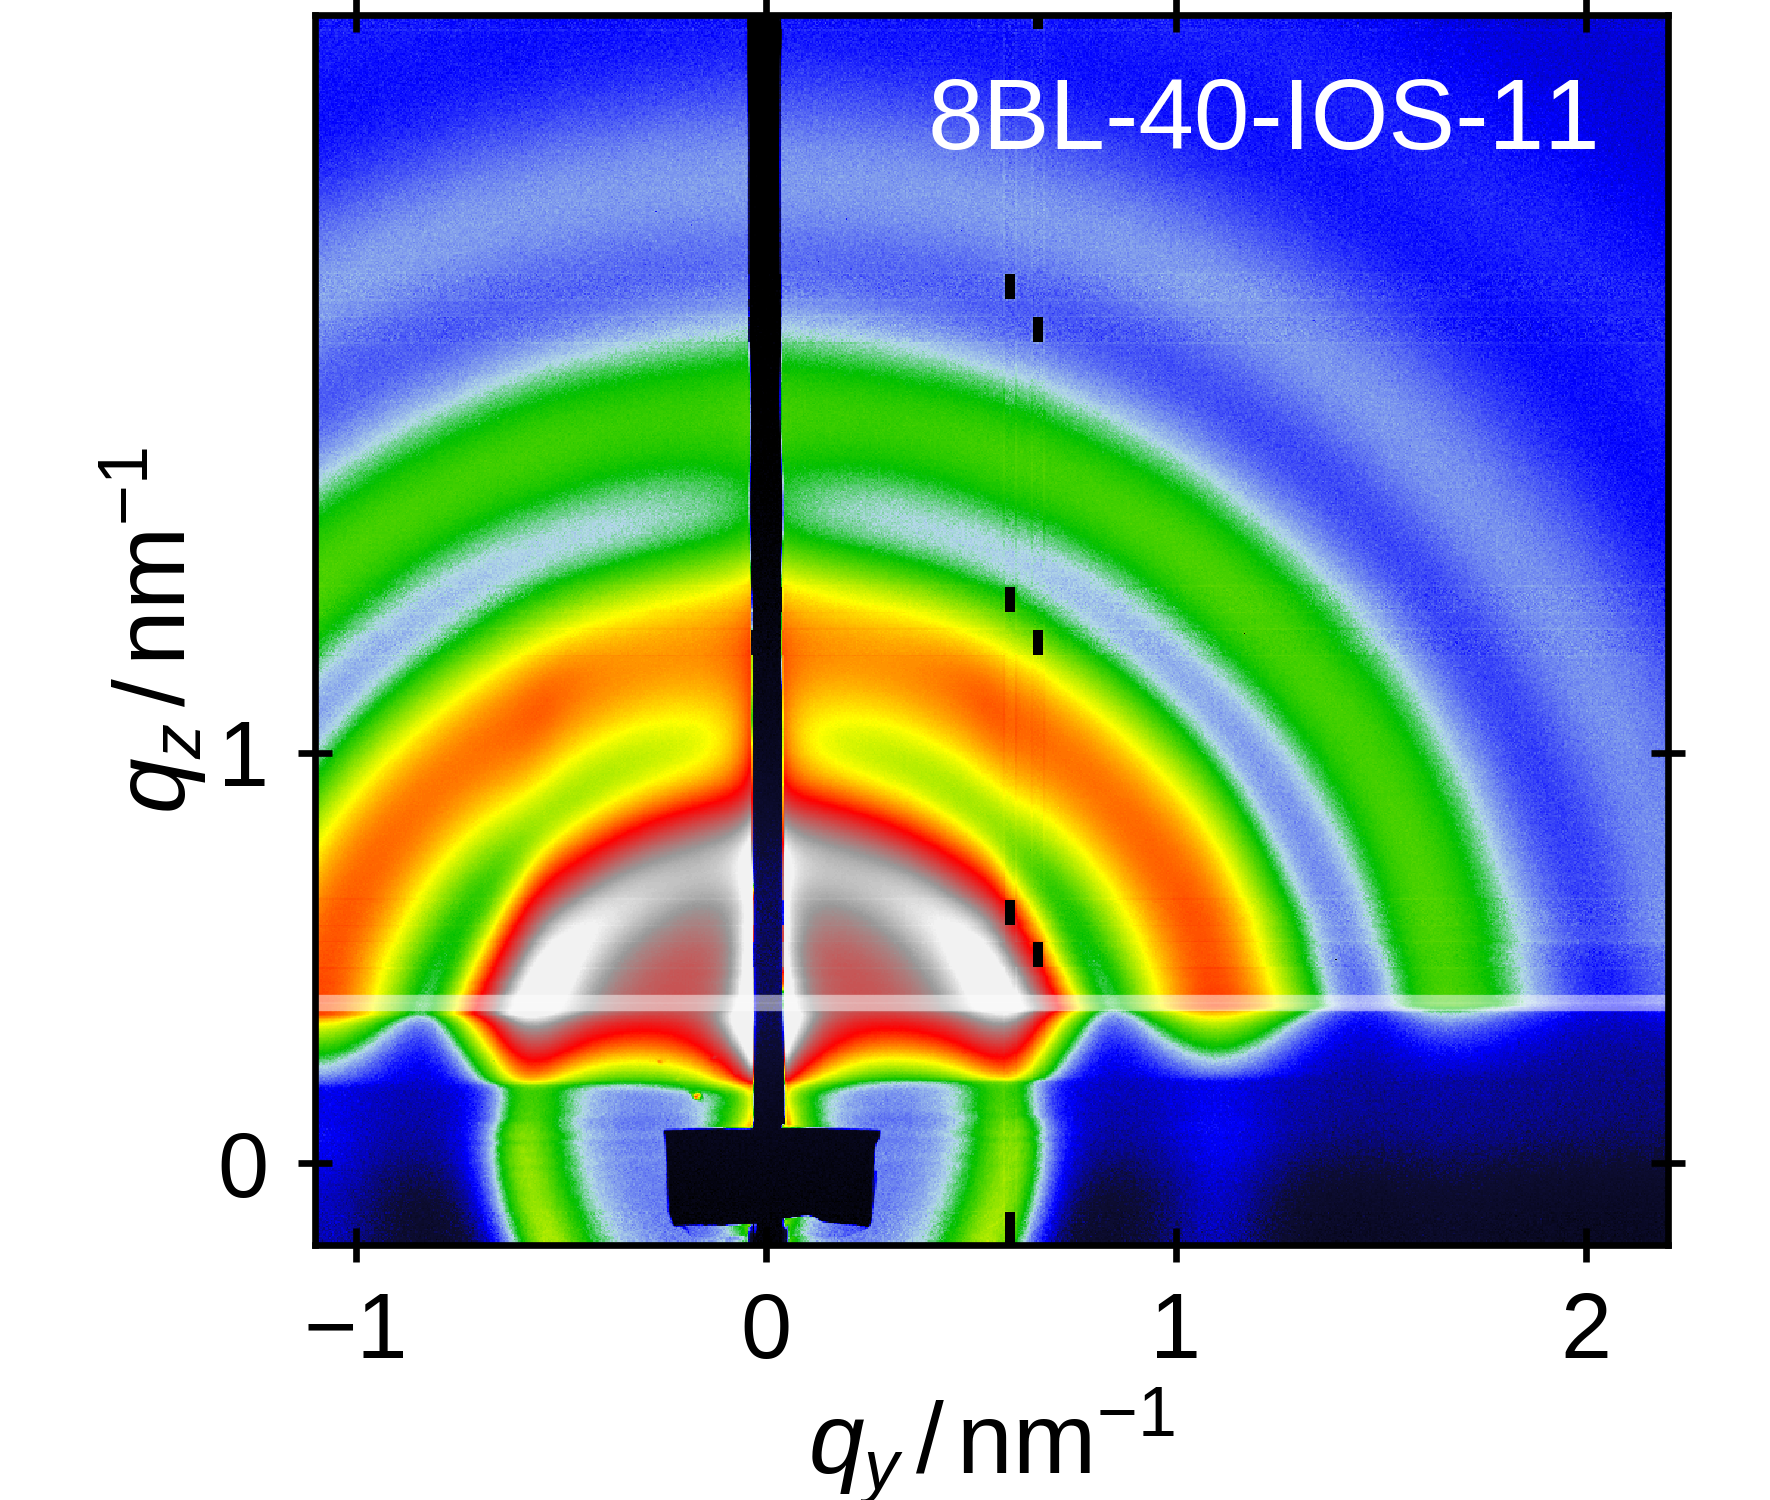
\includegraphics{looselyPackedNP_GISAXS_8BL-40-IOS-11}
    \caption{\label{fig:looselyPackedNP:bilayerStacks:gisaxs8BL_IOS_11}GISAXS detector images (left) of SC-IOS-11 measured under an incident angle of $\alpha_i \eq 0.2 \unit{^\circ}$ and the integrated data in the Yoneda band (right) as blue curve and the previously determined SAXS data (rescaled) for comparison in red. The integrated area for the Yoneda band is shown on the detector image as white stripe. A fit of the intensity using a hard-sphere structure factor in Percus-Yervick approximation, with parameters listed in \reftab{tab:looselyPackedNP:nanoparticle:gisaxs} is shown in black.}
  \end{figure}

  \begin{figure}[tb]
    \centering
    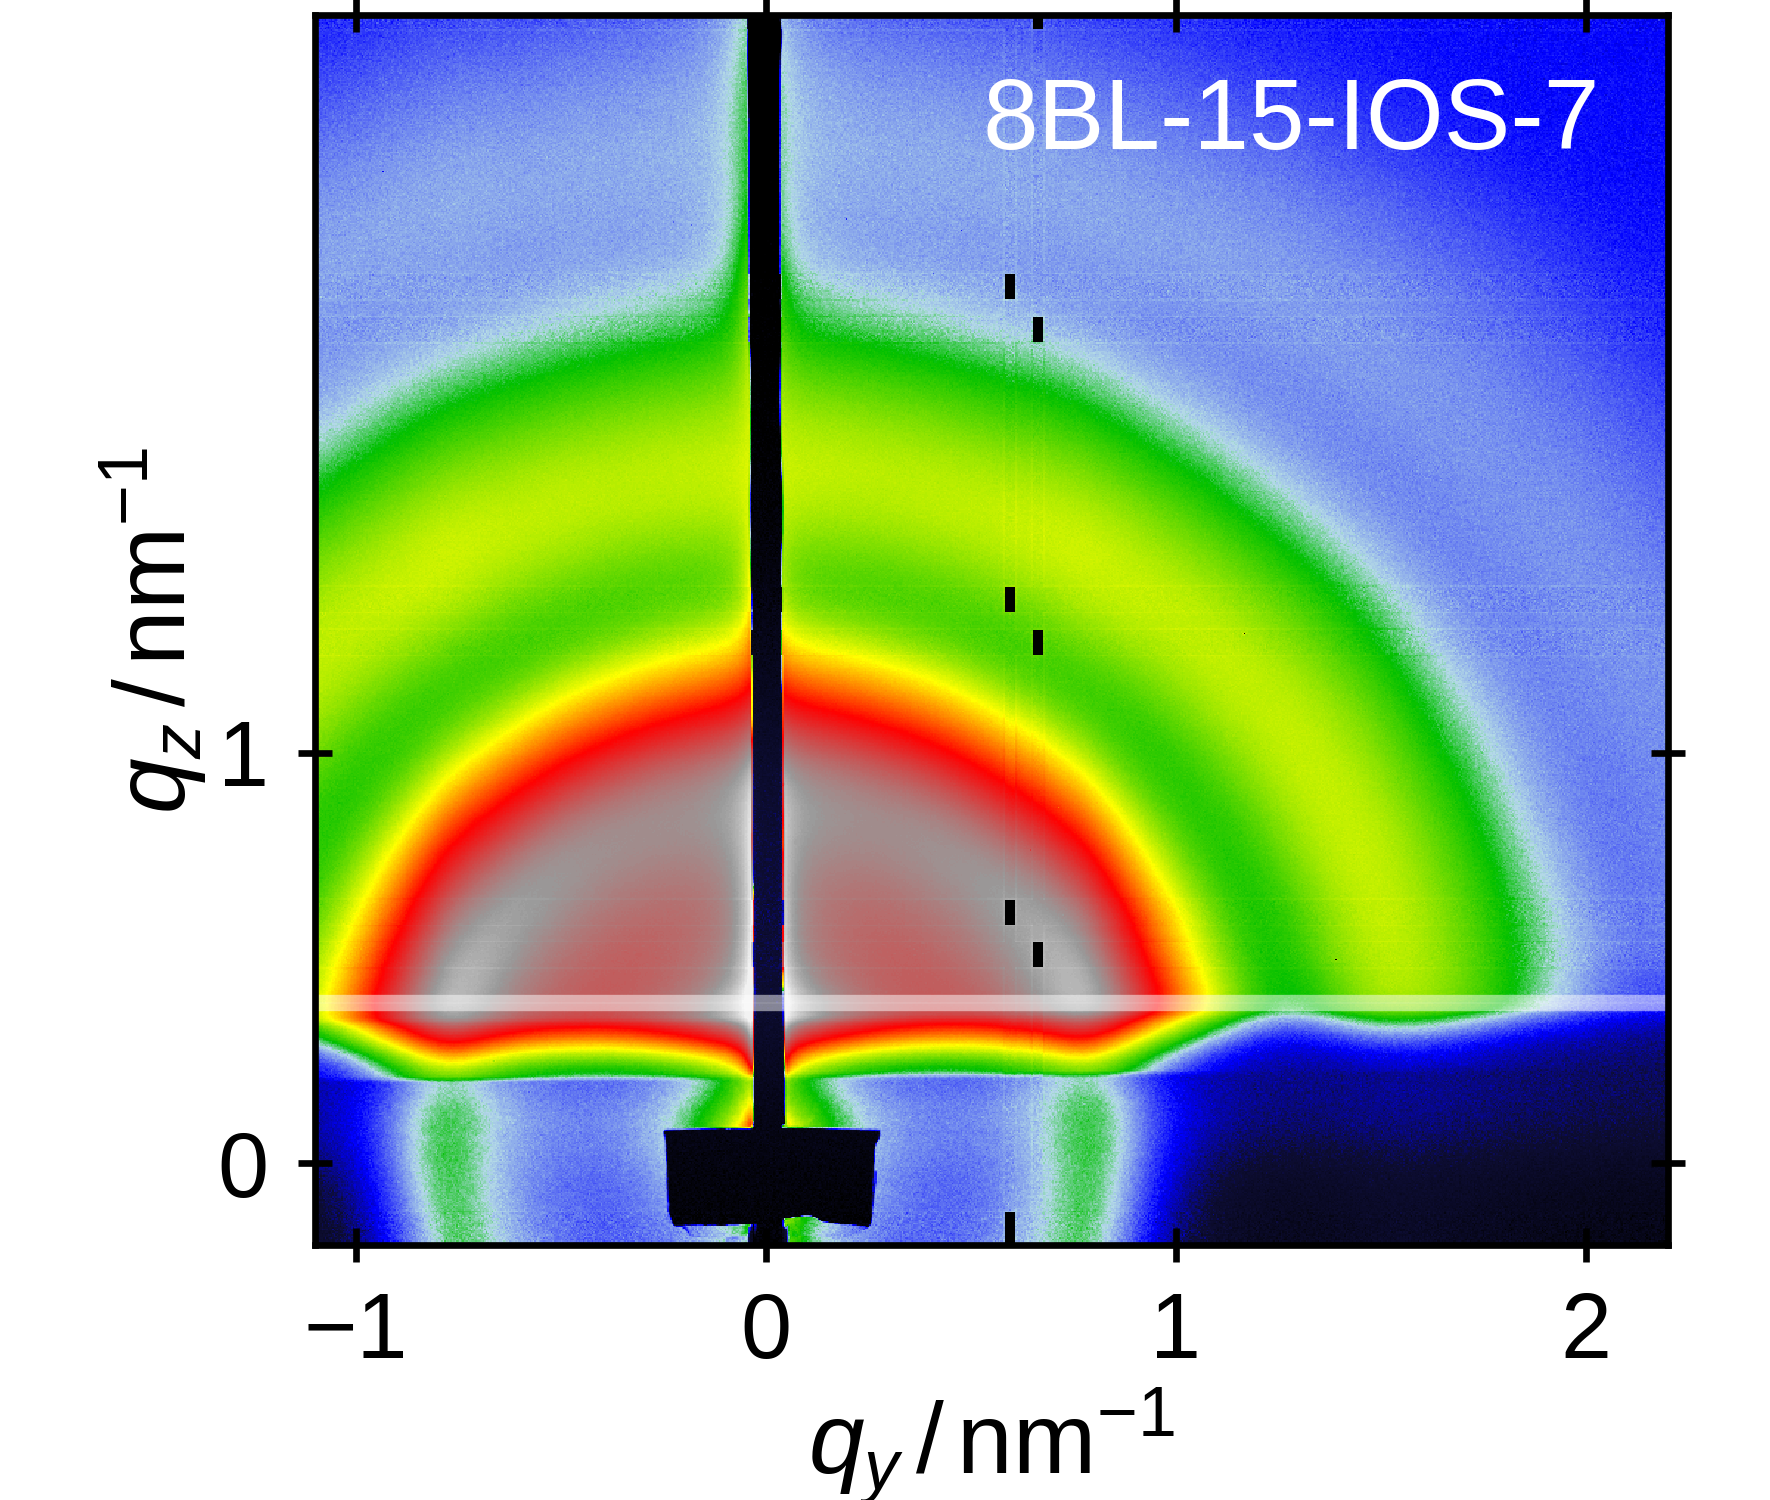
\includegraphics{looselyPackedNP_GISAXS_8BL-15-IOS-7}
    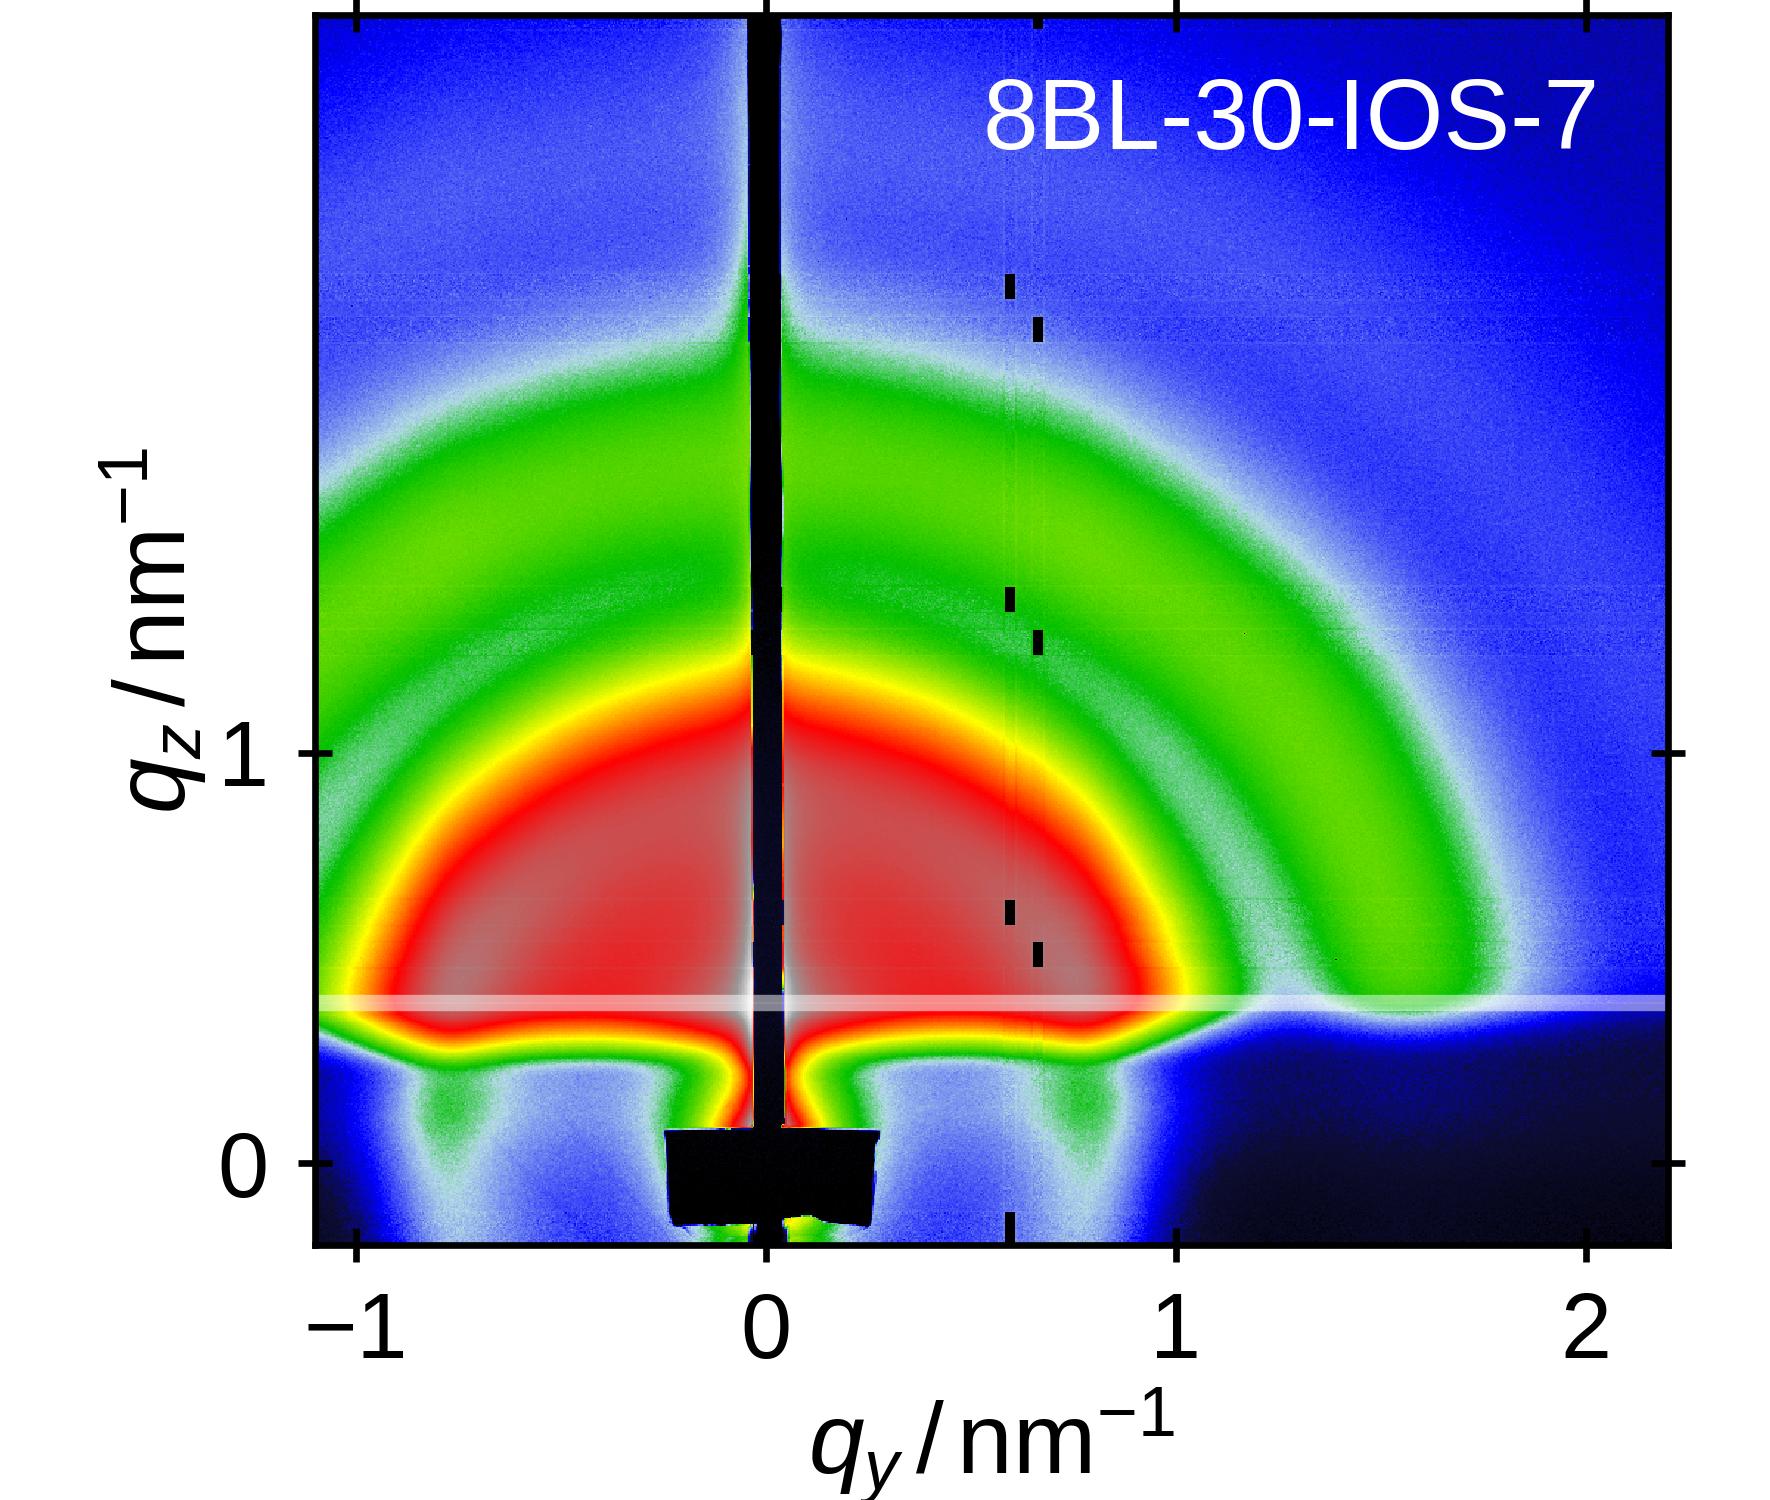
\includegraphics{looselyPackedNP_GISAXS_8BL-30-IOS-7}
    \caption{\label{fig:looselyPackedNP:bilayerStacks:gisaxs8BL_IOS_7}GISAXS detector images (left) of SC-IOS-11 measured under an incident angle of $\alpha_i \eq 0.2 \unit{^\circ}$ and the integrated data in the Yoneda band (right) as blue curve and the previously determined SAXS data (rescaled) for comparison in red. The integrated area for the Yoneda band is shown on the detector image as white stripe. A fit of the intensity using a hard-sphere structure factor in Percus-Yervick approximation, with parameters listed in \reftab{tab:looselyPackedNP:nanoparticle:gisaxs} is shown in black.}
  \end{figure}
  % \begin{table}[tb]
  %   \centering
  %   \caption{\label{tab:looselyPackedNP:nanoparticle:gisaxs}Parameters for the hard-sphere structure factor in Percus-Yervick approximation shown in \reffig{fig:looselyPackedNP:layer:gisaxs} for both SC-IOS-11 and SC-IOS-7. $R_\mathrm{HS}$ is the hard-sphere radius and $\eta$ the packing fraction of the structure factor. Using both values the Wigner-Seitz radius $\bar{r}$ is determined.}
  %   \begin{tabular}{ c | l | l }
  %     \rule{0pt}{2ex} \textbf{GISAXS}  & \textbf{SC-IOS-11} & \textbf{SC-IOS-7} \\
  %     \hline
  %     \rule{0pt}{2ex} $R_\mathrm{HS} \, / \unit{nm}$          & $5.655(2)$           & $3.872(4)$\\
  %     \rule{0pt}{2ex} $\eta          \, / \unit{\%}$          & $43.88(3)$           & $34.20(9)$\\
  %     \hline
  %     \rule{0pt}{2ex} $\bar{r}       \, / \unit{nm}$          & $7.44(1)$            & $5.54(1)$\\
  %     \hline
  %   \end{tabular}
  % \end{table}

\end{document}